\section{Learning traffic patterns}\label{traffic-patterns}
% Why find traffic patterns?
% What is this section for?
% How? --> follows from the subsections.
In order to reason about the traffic in Beijing, and provide some measure of how the previous traffic possibly affects our belief in how the future traffic situation will be in the road network, we analyse the preprocessed data to look for patterns. In this section, we consider methods for extracting such patterns and propose how to apply them on the Bejing dataset.
\subsection{Methods}\label{patterns:methods}
From our knowledge representation of the road network and traffic, we want to predict how traffic affects the travel time of roads in the road network. In order to do this, we need a measure of the traffic on roads. There are several ways one could construct such a measure, incuding
\begin{itemize}
\item \emph{capacity}: How many vehicles can travel on a road, safely, while not negatively affecting the average speed driven on the road?
\item \emph{classification}: Define a class feature of a road, that defines the state of the road. An example could be $Traffic \in \{free, light, medium, heavy\}$. A given road then has a classification based on the observations of speed within some time period.
\item \emph{speed}: we measure the traffic on a given road, by how fast you can drive on the road. In addition, one could measure the ratio between speed and speed limit.
\end{itemize}
The capacity of a road would be possible to estimate from the speed limit, length of a road, safety distances and number of cars. However, drivers do not always drive in a uniform manner, which makes it difficult to accurately estimate capacities.\par
Performing some discrete classification could help to distinguish between different traffic states. Intuitively, a person might be interested in knowing if a road is clear, mildy congested or heavyily congested. Such information could be captured by classifying roads by a roatio between speed limit and actual speed. This raises the questions of which classes should be used and how many. If there are not enough classes, it might be difficult to choose which road to take if both are congested more or less equally.\par

To more easily be able to evaluate roads where traffic is similar, we must use a measure that has a finer granularity. By looking directly at the actual speed driven on roads, we can determine more precisely the costs of taken a particular road. The actual speed, together with the length of a road is also the most important factors in in evaluating the travel time for a road. Therefore, we take a regression approach for predicting traffic.
\subsection{Regression model}\label{patterns:regression-model}
To predict the traffic speed on a given road segment, at a given time we can consider a speed prediction a function:

\begin{align}\label{eq:speed}
speed: E \times T \times W \rightarrow \mathbb{R}
\end{align}
that maps a road segment, time of day and day of week to the a real valued speed prediction. The remaining question is then, how to actually perform the prediction of traffic on a segment given a specific time. \par
Predicting the numeric value of some variable based on previous observations is typically associated with regression. Regression fits input and output pairs to a function, such that future values for input pairs can be predicted. Fitting a regression function on the observations for a particular road segment, provides a way to predict the traffic on the segment. However, since traffic varies over time, one could argue that a polynomial regression function would fit the observations better than a linear function as illustrated in figure \ref{fig:compare-regression}.
\begin{figure}
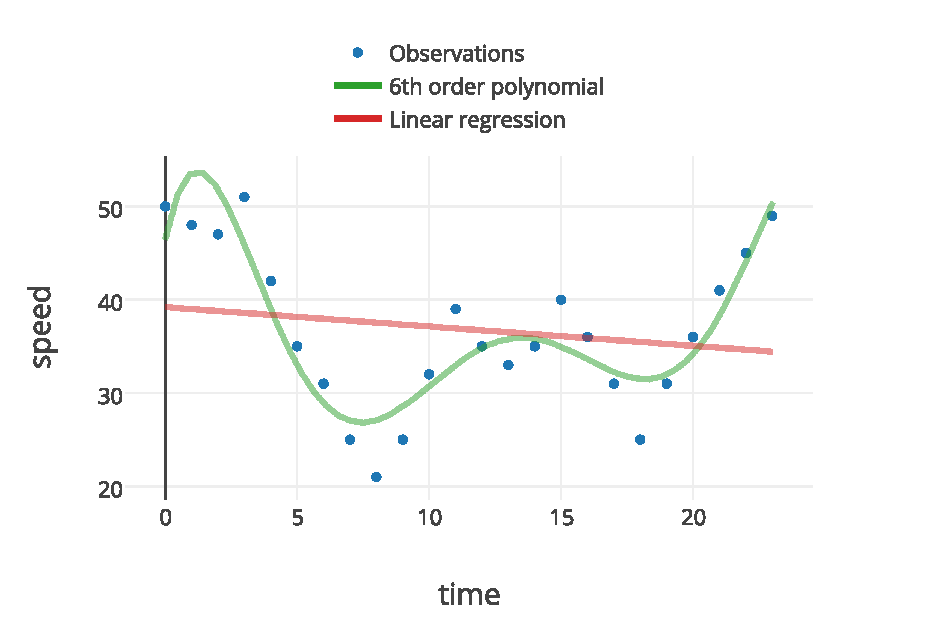
\includegraphics[width=\textwidth]{figures/compare-regression.pdf}
\label{fig:compare-regression}
\caption{Different regression fits on the same dataset.}
\end{figure}
Even though the higher order regression functions generally fits the training data better, such a fit might cause \emph{overfitting} observations, where the accuracy of future predictions decreases and the a linear fit might fit the future observations better. \par
However, a linear regression over the observations for a whole day is not as useful for predicting the fluctuations in traffic during the day, because linear functions by definition cannot model large fluctuations. For this reason, we instead utilise several linear regression models over the course of a day. More specifically, we split a day into partitions $p_1,...,p_i,...,p_n$ where $p_i = (t_1,...,t_j,...,t_k)$ and $t_1,t_2$ are time-stamps. Thus, a partition is defined as a period of time between $t_1$ and $t_2$ that contains every possible timestamp $t_j$ from $t_1$ to $t_k$. For every $p_i$, we perform a linear regression fit, $f_i$, over the observations within that period of time where $f_i:E \rightarrow \mathbb{R}$. In practice, the overall regression function, $speed$, for a road segment becomes a piecewise linear function:
\begin{equation}\label{eq:speed-piecewise}
speed(e,t, w) =
\begin{cases}
f_1(e)       & \quad \text{if } t \in p_1\\
f_2(e)  & \quad \text{if } t \in p_2\\
&\vdots\\
f_n(e) & \quad \text{if } t \in p_n
\end{cases}
\end{equation}

where $f_1,...,f_n$ are linear regression functions for each partition over the observations for segment $e$. The idea is illustrated in Figure \ref{fig:segmented-regression}.
\begin{figure}
\centering
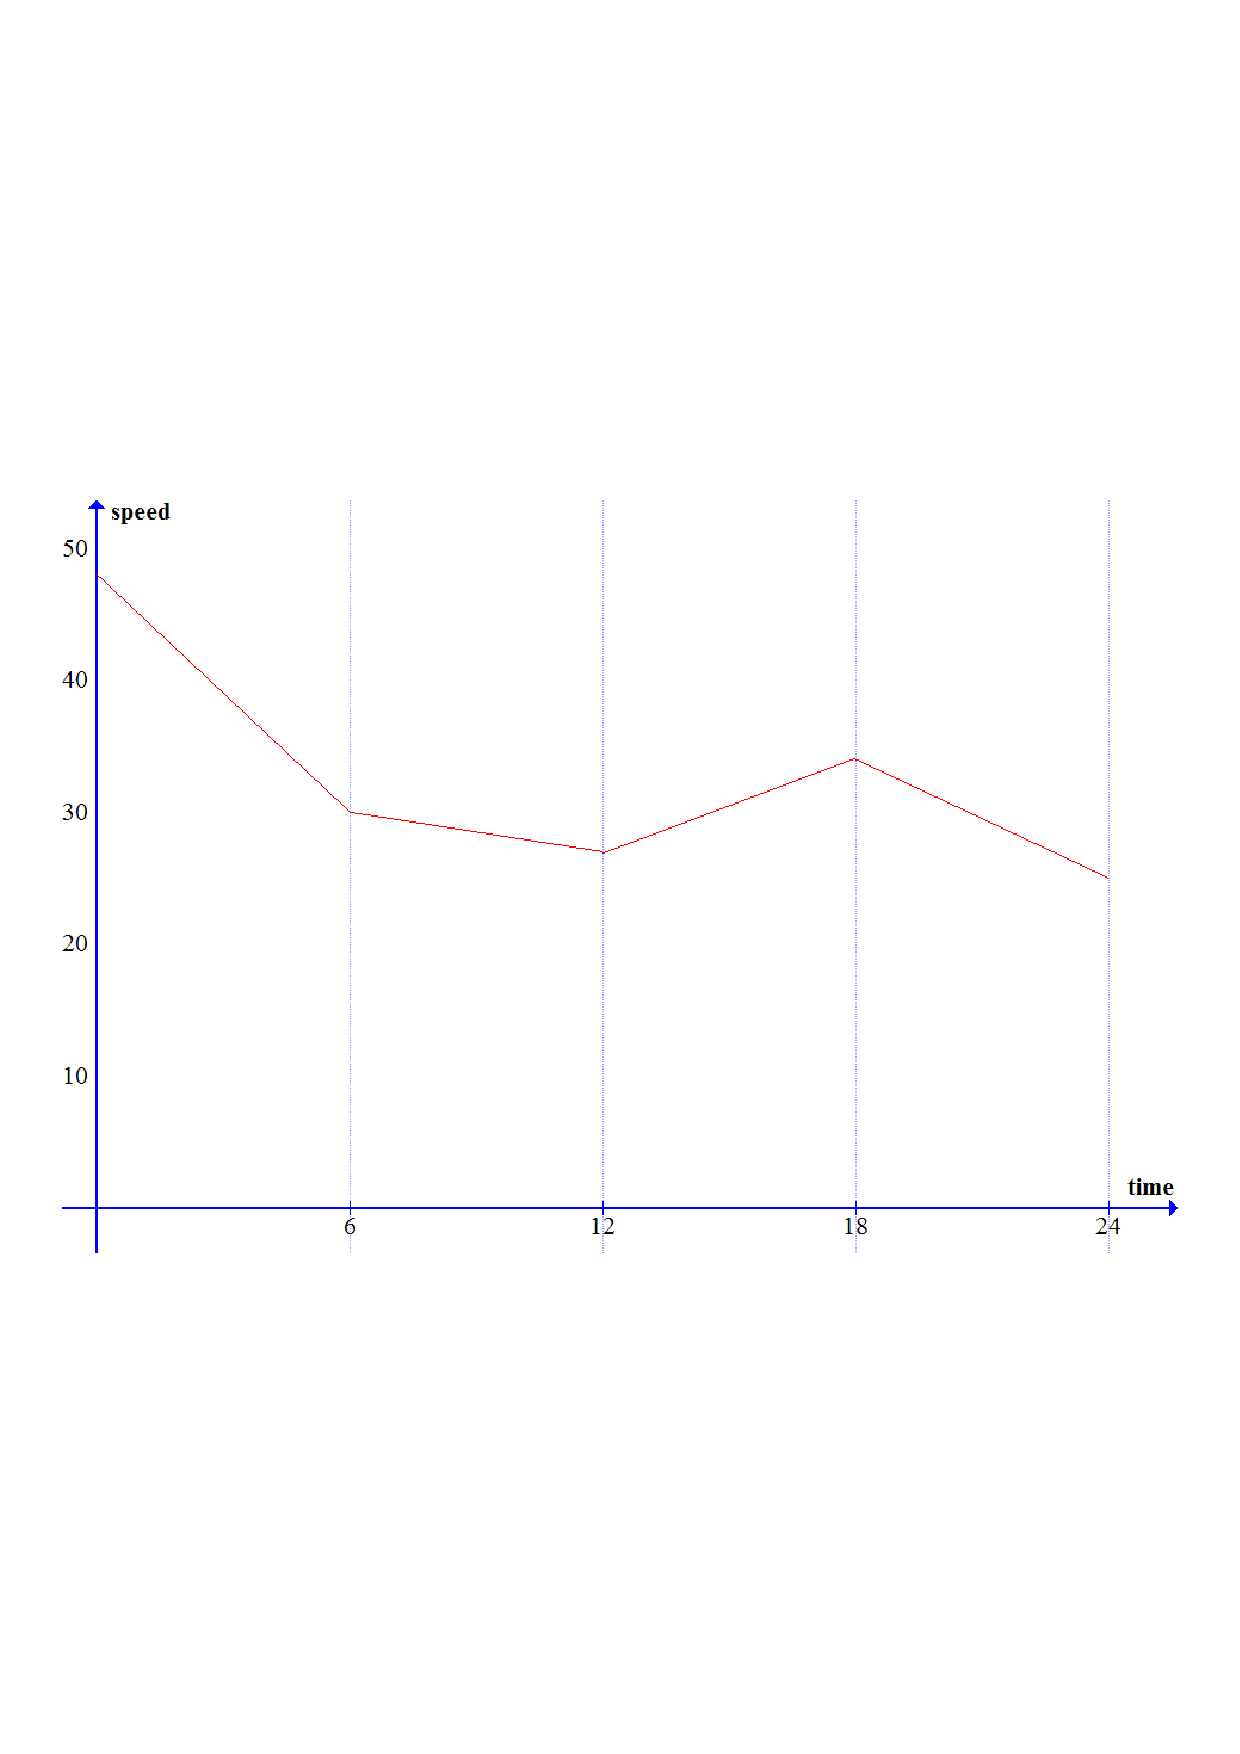
\includegraphics[trim={0 9cm 0 9cm},clip, width=\textwidth]{figures/piecewise.pdf}
\caption{Example of piecewise linear regression - day of 24 hours are partitioned into 4 parts. Every partition has a linear function describing traffic in this time period.}
\label{fig:segmented-regression}
\end{figure}
% Why use it?
% - We want to predict impact of traffic on travel time.
% - How do we measure traffic ?
% 	-	Capacity of roads?
% 		- Difficult to determine accurately, people drive unsafe?
% 	- 	Speeds on roads?
% 	-	Try to classify on congestion?
% 		- k-ary class feature, that classifies a road.
% 		- Penalty of different classes.
% 		- How do we discretize our data into reasonable classes?
% 		- What about roads costs that are almost equal?
% 		- Classes defined by us might not reflect reality.
% 	-	Speed is more "pure" measurement of travel properties of a road
% 		- Speed tells both tells us the penalty of driving on road and has a better granularity of deciding between two almost equal costs of roads.
% 		- Methods for learning traffic:
% 			-	Linear regression
% 			-	Polynomial regression
% 				- Fits the learning data better, but might not fit future samples better! (SSE)
% 			-	But! Traffic also changes over time? (day, week etc..)
% 			-	Divide days into segments, for every segment define fit a linear regression function.
% 			-	How do we segment days?
% 			-	Residual sum
% 			-	Algorithms, M5P automatically splits and generates linear functions
%
% What is it?
% How did we use it?
% Alternatives ?
\\
\subsection{Partitioning scheme}\label{patterns:segmentation}
% Why do it?
%	Want: piecewise linear functions, but how should we partition the days?
In order to use the piecewise linear regression approach, we must devise a partitioning scheme. One such scheme could be the one in Figure \label{fig:segmented-regression} where every day a split into 4 equal partitions: night, morning, afternoon, evening. The following problems are raised by the choice of partitioning scheme:
\begin{itemize}
	\item Where should we split the day, such that important changes in traffic are captured?
	\item How many observations is required to perform regression?
	\item How do we guarantee enough observations in every partition?
\end{itemize}
While it makes sense to have equally sized partitions, it does not guarantee that there will be enough observations to perform a accurate regression for every partition (an example would be, that there are usually less vehicles driving at night, thus less observations in this partition). Furthermore, since traffic patterns most likely are different for different road segments, a static partitioning is not guaranteed to capture important patterns in traffic, such as morning traffic. Therefore, we must incorporate a finer granularity in the partitioning scheme, possibly different for every segment, to capture the differences traffic patterns and to ensure that there will be enough observations to actually perform regression.

This leads us to a dynamic partitioning scheme, where the partitioning is based on the density of observations and how well the function fits the data. A measure to use for such a partitioning, could be the Sum of Squared Errors, which is a measure of how close a predicted value is to the real value. Partitioning is then done, based on minimizing the Sum of Squared Errors, as this yields more accurate regression models.

%\subsection{Quality measure}\label{quality-measure}
%Some of the observations might be based on a small number of GPS samples, or data that is map-matched with a high error rate (accuracy of which road was best to map-match on). Such observations could potentially introduce noise into the regression model and must therefore be taken into account when we construct the model trees. 

%Furthermore, we are interested in weighing the most accurate data higher than data with worse quality, since more accurate data tells us more about the traffic on a given segment. To do that, we introduce a quality measure of observations. The quality measure describes the ratio between the number of GPS samples used to create an observations, and the length of the road segment where the observation was made. That is, the quality measure, $Q$ of an observation, $o$ is given by:
%\begin{equation}
%Q(o) = \frac{|wp|}{|e|}+0.29
%\end{equation}
%where $|e|$ is the length of a road segment $e$, and $|wp|$ is the number of waypoints used to construct $o$.
% Why?
% 	some data might be unreliable, better to use good data first
% What?
% 	We introduce a quality measure --> such that we can decide which observations are "better" in the sense of accuracy observations.
% How?
%	based on the ratio between the length of the segment and the
%	number 	of 	waypoints
% Could also include error rate from mapmatching, but unsure what it means (probably means accuracy of which the mapmatching was done)

\subsection{Model trees}\label{patterns:weka}
% Why use it? (does exactly what we need)
To implement the piecewise regression model described in Section \ref{patterns:regression-model}, we must either construct an algorithm or apply an existing one to the data. One could develop a partitioning scheme and then perform a linear regression on each partition. However, such an approach could potentially yield regression models that does not take into account the growth of predecessor and successor partitions' models. Furthermore, it is not clear how an effective partitioning scheme should be devised, to facilitate dynamic partitioning.

% What is it? (M5P algorithm)
Fortunately, existing work related to the piecewise linear regression model approach exists, in so called \emph{model trees} and \emph{regression trees}. As illustrated in Figure \ref{fig:model-tree}, a \emph{model tree} is a decision tree that has regression models that can either be functions or constants at the leaves. Hence, based on the value of the feature being decided on the model tree has a regression model for any possible world over the set of features. A regression tree is a specialization of a model tree, where the regression models at the leaves are constants.

Several algorithms exist for inducing a piecewise linear regression including \emph{CART}, \emph{M5}, \emph{M5'} - an improved version of M5 - and \emph{MARS} \todo{need refs for these algorithms}. Wang and Witten\cite{IMTCC96} argues, that M5' performs somewhat better than M5 and produces model trees that are more comprehensible due to the size of the trees. Furthermore, open-source implementations of M5' are available for use, which provide a useful basis for inducing model trees for the traffic data.

% How do we use it? (M5p in weka)
For implementing M5' model trees and data filters we use the machine learning tools and algorithm implementations in Weka\cite{Weka}. Weka contains an implementation of the M5' model tree induction algorithm (called M5P in Weka). Weka can be invoked directly from Java code, and therefore integrates well with the rest of the system.

\subsubsection{M5' model tree induction}
% How does it work?
M5' constructs a model tree, like the one illustrated in Figure \ref{fig:model-tree}, from a set of training examples, $T$.
\begin{figure}[H]
	\centering
	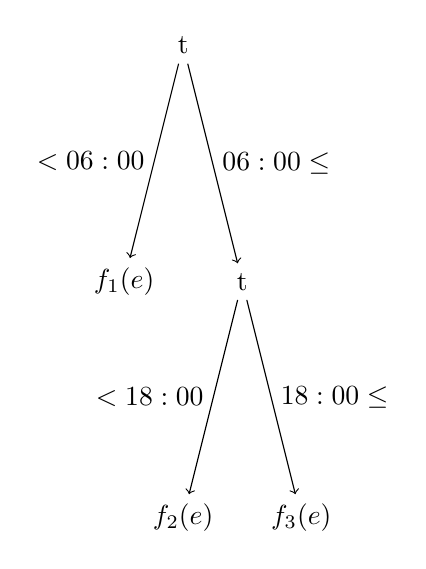
\begin{tikzpicture}
	\node {t}
	[level distance=3cm]
	child { node {$f_1(e)$} edge from parent [->] node [left] {$ < 06:00 $} }
	child { node {t}
		child { node {$f_2(e)$} edge from parent [->] node [left] {$ < 18:00 $}}
		child { node {$f_3(e)$} edge from parent [->] node [right] {$ 18:00 \le $} }
		edge from parent [->] node [right] {$06:00 \le $}
	}
	;
	\end{tikzpicture}
	\caption{Example of a simple model tree with three partitions and three linear regression models. The $t$ feature corresponds to the input time feature in equation \ref{eq:speed-piecewise}}
	\label{fig:model-tree}
\end{figure}
It works by recursively constructing a decision tree by splitting $T$ into subsets $T_1,T_2$ where the split point is determined by examining all possible splits over all non-class features and the domains of those features. The split that yields the highest reduction in standard deviation is chosen at each step.
The resulting tree is then pruned for nodes and leaves that yield a worse standard deviation reduction than parent nodes. This pruning process makes sure the final model is not overfitting the training examples and can better be applied to unseen data. 
Finally, the resulting regression models at the leaves of the tree are mutually smoothed as to minimizes sharp transitions from model to model.

Using this approach, M5' facilitates a dynamic partitioning scheme, based on the measure of standard deviation and smooths transitions between partitions.

\subsection{Generating speed functions}
% Why ?
Using the M5' implementation in Weka, we generate model trees for road segments on a day-by-day basis as described in Section \ref{traffic-patterns}. However several issues are raised about the data used for inducing the model trees:
% What ?
\begin{itemize}
\item Noisy data can skewer the regression models to be inaccurate.
\item Incorrectly mapmatched observations can skewer regression models.
\item Observed speeds above the speed limit introduces the possibility that the system can suggest driving faster than allowed.
\item A segment might not have enough observations to construct a (useful) regression model.
\end{itemize}
% How ?
To minimize the effect of these issues, we perform filtering on the observations based on the \emph{Median Sample Rate} and mapmatching error. Furthermore observations speeds higher than two times the speed limit are filtered, because such high speeds are more likely to be noise data. Observations with speeds between 100\% to 200\% the speed limit are lowered to the max speed, since such observations might be realistic, but we still do not want them to affect the regression model.

Additional thresholds for filters can be seen in \tabref{tab:datafiltering} (the green row is the one we use).
%  SELECT COUNT(o.*) FROM Observations o, Segments s, Ways w, Roadtypes t WHERE o.speed > 1 AND o.speed < t.speedlimit * 2 AND o.length > 0.005 AND o.mediansamplerate <= 20 AND o.error < 100 AND numwaypoints > 4 AND o.segment = s.id AND s.way = w.id AND w.type = t.id;
\begin{table}[H]
	\centering
	\begin{tabular}{TlTlTlTlTlTlT}
		\thickhline
		\textbf{Speed}                                                                          & \textbf{Length}  & \textbf{MSR}  & \textbf{MME} & \textbf{\#Wpts} & \textbf{Observations} \\ \thickhline
		-                                                                                       & -                & -             & -              & -               & 4584306               \\ \thickhline
		\begin{tabular}[c]{@{}l@{}}\textgreater 1 km/h\\ \textless speed limit * 2\end{tabular} & \textgreater 5 m & \textless= 20 & \textless 100  & \textgreater= 5 & 269527                \\ \thickhline
		\begin{tabular}[c]{@{}l@{}}\textgreater 1 km/h\\ \textless speed limit * 2\end{tabular} & \textgreater 5 m & \textless= 20 & \textless 100  & -               & 867128                \\ \thickhline
		\begin{tabular}[c]{@{}l@{}}\textgreater 1 km/h\\ \textless speed limit * 2\end{tabular} & -                & \textless= 20 & \textless 100  & -               & 878426                \\ \thickhline
		\textless speed limit * 2                                                               & -                & \textless= 20 & \textless 100  & -               & 898774                \\ \thickhline
		\textless= speed limit                                                                  & -                & \textless= 20 & \textless 100  & -               & 861766                \\ \thickhline
		\textless= speed limit                                                                  & -                & \textless 300 & \textless 100  & -               & 2861949               \\ \thickhline
		\rowcolor[HTML]{34FF34}
		\begin{tabular}[c]{@{}l@{}}\textgreater 1 km/h\\ \textless speed limit * 2\end{tabular} & \textgreater 5m  & \textless= 60 & \textless 100  & -               & 1715070               \\ \thickhline
		\begin{tabular}[c]{@{}l@{}}\textgreater 1 km/h\\ \textless speed limit * 2\end{tabular} & \textgreater 5m  & \textless= 60 & \textless 100  & \textgreater= 3 & 913779                \\ \thickhline
	\end{tabular}
	\caption{Observations remaining after using various filters. MSR = median sample rate of the link, \#Wpts = number of waypoints in the link.}
	\label{tab:datafiltering}
\end{table}
	\todo{make percent of how many observations (in table) are filtered. Benjamin }
\emph{MSR} is the median sample rate calculated using only waypoints that are at least 1.4 metres apart, \emph{\#Wpts} is the total number of waypoints on the link, \emph{Length} is the distance driven between the first and the last waypoint in the link, and \emph{Observations} is the number of observations remaining after applying the filters.
The tresholds are based on informal study of how high requirements of MSR and MME (mapmatching error) was possible, without discarded too much data.
Additionally, we perform normalisation of the timestamps of observations, due to Weka3's internal representation of time being problematic when doing regression.